%%%%%%%%%%%%%%%%%%%%%%%%%%%%%%%%%%%%%%%%%%%%%%%%%%%%%%%%%%%%%%%%%%
%%%%%%%% ICML 2015 EXAMPLE LATEX SUBMISSION FILE %%%%%%%%%%%%%%%%%
%%%%%%%%%%%%%%%%%%%%%%%%%%%%%%%%%%%%%%%%%%%%%%%%%%%%%%%%%%%%%%%%%%

% Use the following line _only_ if you're still using LaTeX 2.09.
%\documentstyle[icml2015,epsf,natbib]{article}
% If you rely on Latex2e packages, like most moden people use this:
\documentclass[10pt]{article}

% use Times
\usepackage{times}
% For figures
\usepackage{graphicx} % more modern
%\usepackage{epsfig} % less modern
\usepackage{float}

% For citations
\usepackage{natbib}

% For algorithms
\usepackage{algorithm}
\usepackage{algorithmic}
\usepackage{bm}
\usepackage{amssymb,amsmath}


% As of 2011, we use the hyperref package to produce hyperlinks in the
% resulting PDF.  If this breaks your system, please commend out the
% following usepackage line and replace \usepackage{icml2015} with
% \usepackage[nohyperref]{icml2015} above.
\usepackage{hyperref}

% Packages hyperref and algorithmic misbehave sometimes.  We can fix
% this with the following command.
\newcommand{\theHalgorithm}{\arabic{algorithm}}

% Employ the following version of the ``usepackage'' statement for
% submitting the draft version of the paper for review.  This will set
% the note in the first column to ``Under review.  Do not distribute.''
\usepackage[accepted]{icml2015}
\usepackage{amsmath}
\usepackage{amsmath}
\usepackage{amsfonts}
\usepackage{amssymb}

\usepackage{todonotes}

\usepackage{amsbsy}

% Employ this version of the ``usepackage'' statement after the paper has
% been accepted, when creating the final version.  This will set the
% note in the first column to ``Proceedings of the...''
%\usepackage[accepted]{icml2015}


% The \icmltitle you define below is probably too long as a header.
% Therefore, a short form for the running title is supplied here:

% Saving space by deleting running title (does this actually save space?)
%\icmltitlerunning{Submission and Formatting Instructions for ICML 2015}

\begin{document} 

\twocolumn[

% Saving space by deleting title
%\icmltitle{Submission and Formatting Instructions for \\ 
%           International Conference on Machine Learning (ICML 2015)}

% It is OKAY to include author information, even for blind
% submissions: the style file will automatically remove it for you
% unless you've provided the [accepted] option to the icml2015
% package.


% You may provide any keywords that you 
% find helpful for describing your paper; these are used to populate 
% the "keywords" metadata in the PDF but will not be shown in the document
\icmlkeywords{6.867, machine learning}

\vskip 0.3in
]

% Saving space by deleting abstract
%\begin{abstract} 
%The purpose of this document is to provide both the basic paper template and
%submission guidelines.
%\end{abstract} 

\section*{Neural Networks}

We implemented a simple 2-layer regularized neural network, trained it using gradient descent, and used it on the provided toy datasets and MNIST handwritten digits datasets.

We choose to use the softmax formulation as described by Bishop for our loss function.  Please note that although this is a different loss function than we were asked to use in our assignment description, there was a follow-up discussion on Piazza (see note @504 if not familiar) which clarified that softmax is actually the correct formulation for 1-of-K classification.

The likelihood according to softmax is:
%
%
\begin{equation}
p(\mathbf{t} \ | \ \mathbf{X}, \mathbf{w}) = \prod_{k=1}^K \prod_{n=1}^N y_k(\mathbf{x}_n,\mathbf{w})^{t_{nk}}
\end{equation}
%
%
And taking the negative log likelihood we have our unregularized loss function:
%
%
\begin{equation}
l(\mathbf{w})= - \sum_{k=1}^K \sum_{n=1}^N  t_{nk} \ln y_k(\mathbf{x}_n,\mathbf{w}) 
\end{equation}
%
%
We note that $\mathbf{w}$ can be considered a vector that represents all of the weights of the neural network, but it is preferable to think of the weights as being organized into two matrices, which we denote $W^{(1)}$ and $W^{(2)}$ and explain later in the context of forward propagation.  The matrix representation, however, is useful for including regularization in our final cost function, which is formulated via the Frobenius norm:
%
%
\begin{equation}
J(w) = l(w) + \lambda(||W^{(1)}||^2_F + ||W^{(2)}||^2_F)
\end{equation}
%
%

\subsection*{Gradient Calculation}

Having defined our cost function, we are now able to describe how the gradients $\nabla_{W^{(1)}} J(\mathbf{w})$ and $\nabla_{W^{(1)}} J(\mathbf{w})$ may be calculated analytically.  Before this derivation, however, we note for clarity that each of these terms are matrices whose elements are simply the partial derivative of the cost function with respect to that element itself (a scalar).

In order to calculate the gradients, we will use error backpropagation, for which we will follow Bishop's nice explanation and follow these sequence of steps:

\begin{enumerate}
 \item Forward propagation
 \item Evaluate $\delta$ for the output units
 \item Backpropagation of the $\delta$'s for each hidden unit
 \item Evaluate derivatives with $\frac{\partial E_n}{\partial w_{ji}}$
\end{enumerate}

\textit{1. Forward propagation}

With the weights represented as matrices, we can vectorize the computation of the unit activations, for example for the first layer:
%
%
\begin{equation}
A^{(1)} = W^{(1)} X_{aug}
\end{equation}
%
%
Where $X_{aug}$ is a $(D+1) \times N$ augmented matrix for the input data, for the purpose of including the bias input unit in the vectorized computation.  If we consider the original input data to be $X$, of dimension $D \times N$, where $D$ is the dimensionality of each sample input and $N$ is the number of sample inputs, then we form $X_{aug}$ by augmenting $X$ with a $1 \times N$ vector of 1s ($X_{aug} = \begin{bmatrix} 1_{N \times 1} &| & X^T\end{bmatrix} ^T$).  $W^{(1)}$ is then a $M \times (D+1)$ matrix that contains all of the weights from every input to every hidden unit, except the hidden bias unit, and $A^{(1)}$ is a $M \times N$ matrix where each column vector is individually the weights for all of the unit activations, given one sample input.  The "output" of each unit is computed simply by applying the sigmoid function $g()$ element-wise to the matrix $A^{(1)}$:
%
%
\begin{equation}
Z^{(1)}_{ij} = g(A^{(1)}_{ij})
\end{equation}
%
%
Where as requested in the assignment, we use the logistic sigmoid function as our sigmoid function:
%
%
\begin{equation}
g(z) = \frac{1}{1 + e^{-z}}
\end{equation}
%
%
To forward propagate through the second layer to the output units, we similarly use $A^{(2)} = W^{(2)} Z_{aug}^{(1)}$, where $Z^{(1)}$ has been augmented with a vector of 1s to include the bias unit, and so we have $W^{(2)}$ of dimension $K \times (M+1)$.  At this point we also note that in order to do our 1-of-K classification, we have to transform the output from the form they were given in the assigned datasets, from a scalar $k$ to $\mathbf{e}_k$ where $\mathbf{e}_k$ is a vector of length $K = k_{max}$ and contains a 0 for every element except $k$, for example if $k=3$ then we form $e_3 = [0 \ 0 \  1]$.  Thus we consider $\mathbf{t}$ to be an $K \times N$ matrix.  Applying $y_{ij} = g(A^{(2)}_{ij})$, we have our outputs and have completed forward propagation.

\textit{2. Evaluate $\delta_k$ for the output units}

With our softmax formulation.... 

... we end up with:
%
%
\begin{equation}
\delta_{nk} = y_{nk} - t_{nk}
\end{equation}
%
%

Which is simply vectorized by element-wise subtraction of $K \times N$ matrices: $\delta = \mathbf{y} - \mathbf{t}$.



\textit{3. Backpropagation of the $\delta$'s for each hidden unit}

Having calculated the $\delta$'s for the output unit, we have only one step of backpropagation to perform, since we have only a 2-layer neural network.  We first provide the backpropagation formula, unvectorized:
%
%
\begin{equation}
\delta_j = g'(a_j)\sum_k w_{kj} \delta_k
\end{equation}
%
%
where $g'(z)=g(z)(1-g(z))$ signifies the gradient of our sigmoid function. We may start vectorizing this computation so that $\delta$ is an $M \times 1$ vector and we have:
%
%
\begin{equation}
\delta_{hidden} = g'(A^{(1)}) * W^{(2)^T}_{\text{no bias}} \delta_{outputs}
\end{equation}
%
%
In the above, $*$ is used to signify element-wise multiplication, and $W^{(2)^T}_{\text{no bias}}$ is a transposed matrix of $W^{(2)}$ except without the vector that corresponds to the bias units.  The above equation holds for calculating $\delta_{hidden}$ for one sample at a time, but also equivalently holds for batch computation $N$ at a time, just by using $\delta_{outputs}$ as a $K \times N$ matrix from step 2, with $W^{(2)^T}_{\text{no bias}}$ of dimension $M \times K$, and $A^{(1)}$ of dimension $M \times N$.

\textit{4. Evaluate derivatives with $\frac{\partial E_n}{\partial w_{ji}}$}

Finally, we use both $\delta$'s together with our inputs, $\mathbf{x}$, and our hidden unit outputs, $Z^{(1)}$, to calculate the gradients $\nabla_{W^{(1)}} J(\mathbf{w})$ and $\nabla_{W^{(1)}} J(\mathbf{w})$.

Following Bishop, we know that we can compute the derivative with respect to any element via:
%
%
\begin{equation}
\frac{\partial J_n}{\partial w_{ji}} = \delta_j z_i
\end{equation}
%
%
In the above, $\delta$ represents the $\delta$ at the output of the weight, and $z$ represents the activation at the input of the weight.  The above only calculates the gradient for one sample, and for one element of the matrix, but to vectorize, we this can be vectorized as:
%
%
\begin{equation}
\nabla_{W^{(1)}} J(\mathbf{w}) = \delta_{outputs} Z^{(1)^T}
\end{equation}
%
%
\begin{equation}
\nabla_{W^{(2)}} J(\mathbf{w}) = \delta_{hidden} X^T
\end{equation}
%
%
where we have explicitly calculated for the gradients with respect to each of the matrices.


\subsection*{Implementing 2-Layer Neural Network}

\subsection*{Stochastic Gradient Descent}
The implementation of stochastic gradient descent (SGD) only requires a small modification to the existing code. In particular if we define
%
%
\begin{equation}
E_n(\mathbf{w}) = -\sum_k t_{n,k} \log(y_k(\mathbf{x}_n,\mathbf{w}))
\end{equation}
%
we can write the objective function as 
%
%
\begin{align}
l(w) &= \sum_n \left[ E_n(w) + \frac{\lambda}{N} (||W^{(1)}||^2_F + ||W^{(2)}||^2_F) \right] \\
& = \sum_n l_n(w)
\end{align}
%
%
Computing the gradient of $l_n(w)$ is fundamentally no different than in the standard case. The only difference is that we only forward/backward propagate for a single sample $x_n$. Thus the computation is much faster than the full gradient computation which takes $N$ times as long, where $N$ is the number of training examples. The other thing we need to define is the learning rate $\eta_n$. The only requirement is that the learning rate satisfy the Robbins-Munro condition. That is $\sum_n \eta_n = \infty, \sum_n \eta_n^2 < \infty$. Following the discussion on Piazza we choose
%
%
\begin{equation}
\eta_n = \frac{\alpha}{{\beta + n}^\gamma}
\end{equation}
%
%
where $\gamma > 0.5$ ensures the Robbins-Munro condition is satisfied. The actual SGD algorithm simply updates the weights $W$ as 
%
%
\begin{equation}
W^{(j+1)} = W^{(j)} - \eta_j \frac{\partial l_{n_j}}{\partial W}|_{W^{(j)}}
\end{equation}
%
%
here $n_j \in \{1,\ldots,N\}$ is the index of the training point used in the $j^{th}$ step of the SGD algorithm. To choose $n_j$ we randomly shuffle the values $\{1,\ldots,N\}$ and loop through them until convergence. The convergence criterion for SGD is also slightly different. The standard convergence criterion requires evaluating the full cost function $l(w)$ at each iteration. Since the whole point of SGD is to avoid doing this, we propose an alternate convergence criterion. In particular we converge when $||W^{(j+1)} - W^{(j)}||$ is sufficiently small. 





\subsection*{Testing the Neural Network Code}



In practice it was necessary to use a relatively large step size $\eta_n$ to get rapid convergence. This makes sense since we expect that the gradient of $l_n(w)$ is about $1/N$ as large as the gradient of $l(w)$. For the toy dataset we used a step size of $N*20 = 6000$ and $\lambda = 0$. In order to get good performance, we set the maximum number of iterations to $50,000$. As can be seen in Figure \ref{SGD_toy_data_2_CER} the performance of stochastic gradient descent is comparable, just slightly worse, than that of the batch method. Cross validation shows that 60 hidden nodes provides the best performance on the test set. However, as can be seen from the figure, we already get good performance with 20 hidden nodes, and that increasing the number of hidden nodes beyond that doesn't yield large gains. However, as Figure \ref{SGD_toy_data_2_training_time} shows, the runtime increases as we increase the number of hidden nodes. This makes sense, since as we increase the number of hidden nodes, we effectively increase the size of the matrices we must multiply together to compute the backpropagation step.

\begin{figure}
\centering
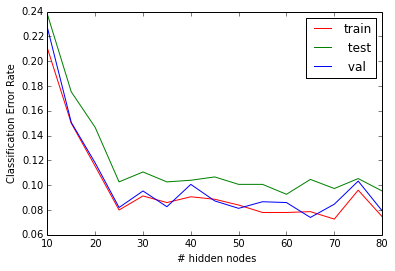
\includegraphics[scale=0.5]{SGD_toy_data_2_CER.png}
\caption{The classification error rate on the train, test and validation datasets for different numbers of hidden nodes}
\label{SGD_toy_data_2_CER}
\end{figure}

\begin{figure}
\centering
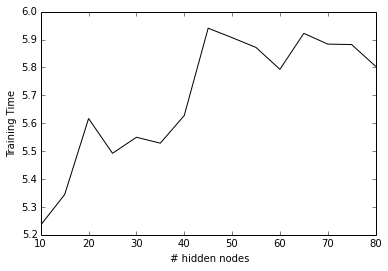
\includegraphics[scale=0.5]{SGD_toy_data_2_training_time.png}
\caption{The classification error rate on the train, test and validation datasets for different numbers of hidden nodes}
\label{SGD_toy_data_2_training_time}
\end{figure}

\subsection*{Testing the Neural Network Code}

\subsubsection*{Stochastic Gradient Descent}
For stochastic gradient descent we again found that a step size of $N*20$ where $N$ is the number of samples works well. Some experimentation showed that between $30$ and $70$ hidden units provided the best performance. We also found that regularization values around $\lam = 2$ provided good generalization performance. In Figure \todo{ref} we plot the classification error rate against the number of hidden units, fixing $\lambda = 2$.
\subsection*{MNIST Data (Parts 5 and 6)}



\end{document} 


% This document was modified from the file originally made available by
% Pat Langley and Andrea Danyluk for ICML-2K. This version was
% created by Lise Getoor and Tobias Scheffer, it was slightly modified  
% from the 2010 version by Thorsten Joachims & Johannes Fuernkranz, 
% slightly modified from the 2009 version by Kiri Wagstaff and 
% Sam Roweis's 2008 version, which is slightly modified from 
% Prasad Tadepalli's 2007 version which is a lightly 
% changed version of the previous year's version by Andrew Moore, 
% which was in turn edited from those of Kristian Kersting and 
% Codrina Lauth. Alex Smola contributed to the algorithmic style files.  
